%\documentclass[paper]{geophysics}
\documentclass[manuscript,endfloat]{geophysics}
\usepackage{graphicx}
\usepackage{subfigure}

% An example of defining macros
\newcommand{\rs}[1]{\mathstrut\mbox{\scriptsize\rm #1}}
\newcommand{\rr}[1]{\mbox{\rm #1}}

\begin{document}

\title{An example \emph{Geophysics} article, \\ with a two-line title}

\renewcommand{\thefootnote}{\fnsymbol{footnote}} 

\address{
\footnotemark[1]BP UTG, \\
200 Westlake Park Blvd, \\
Houston, TX, 77079 \\
\footnotemark[2]Bureau of Economic Geology, \\
John A. and Katherine G. Jackson School of Geosciences \\
The University of Texas at Austin \\
University Station, Box X \\
Austin, TX 78713-8924}
\author{Joe Dellinger\footnotemark[1] and Sergey Fomel\footnotemark[2]}

\footer{Example}
\lefthead{Dellinger \& Fomel}
\righthead{\emph{Geophysics} example}

\maketitle

\begin{abstract}
  This is an example of using \textsf{geophysics.cls} for writing
  \emph{Geophysics} papers.
\end{abstract}

\section{Introduction}

This is an introduction. \LaTeX\ is a powerful document typesetting
system \cite[]{lamport}. An excellent reference is \cite[]{kopka}. The
new \textsf{geophysics.cls} class complies with the \LaTeX2e\
standard.

\section*{Theory}

This is another section. 

\subsection{Equations}

Section headings should be capitalized. Subsection headings should only
have the first letter of the first word capitalized.

Here are examples of equations involving vectors and tensors:
\begin{equation}
\tensor{R} = \pmatrix{R_{\rs{XX}} & R_{\rs{YX}} \cr R_{\rs{XY}} & R_{\rs{YY}}} 
=
\tensor{P}_{M\rightarrow R} \; \tensor{D} \; \tensor{P}_{S\rightarrow M}
\;\;\; \tensor{S} \ \ \  ,
\label{SVD}
\end{equation}
and
\begin{equation}
R_{j,m}(\omega) =
\sum_{n=1}^{N} \, \,
P_{j}^{(n)}(\mathbf{x}_R) \, \,
D^{(n)}(\omega) \, \,
P_{m}^{(n)}(\mathbf{x}_S) \ \ \ .
\label{SVDray}
\end{equation}

Note that the macro for the \verb#\tensor# commands has been changed
to force tensors to be bold uppercase, in compliance with current SEG
submission standards. This is so that documents typeset to the old
standards will print out according to the new ones: e.g., tensor
$\tensor{t}$ (note converted to uppercase).

\subsection*{Figures}

Figure~\ref{fig:waves} shows what it is about.

\begin{figure}
  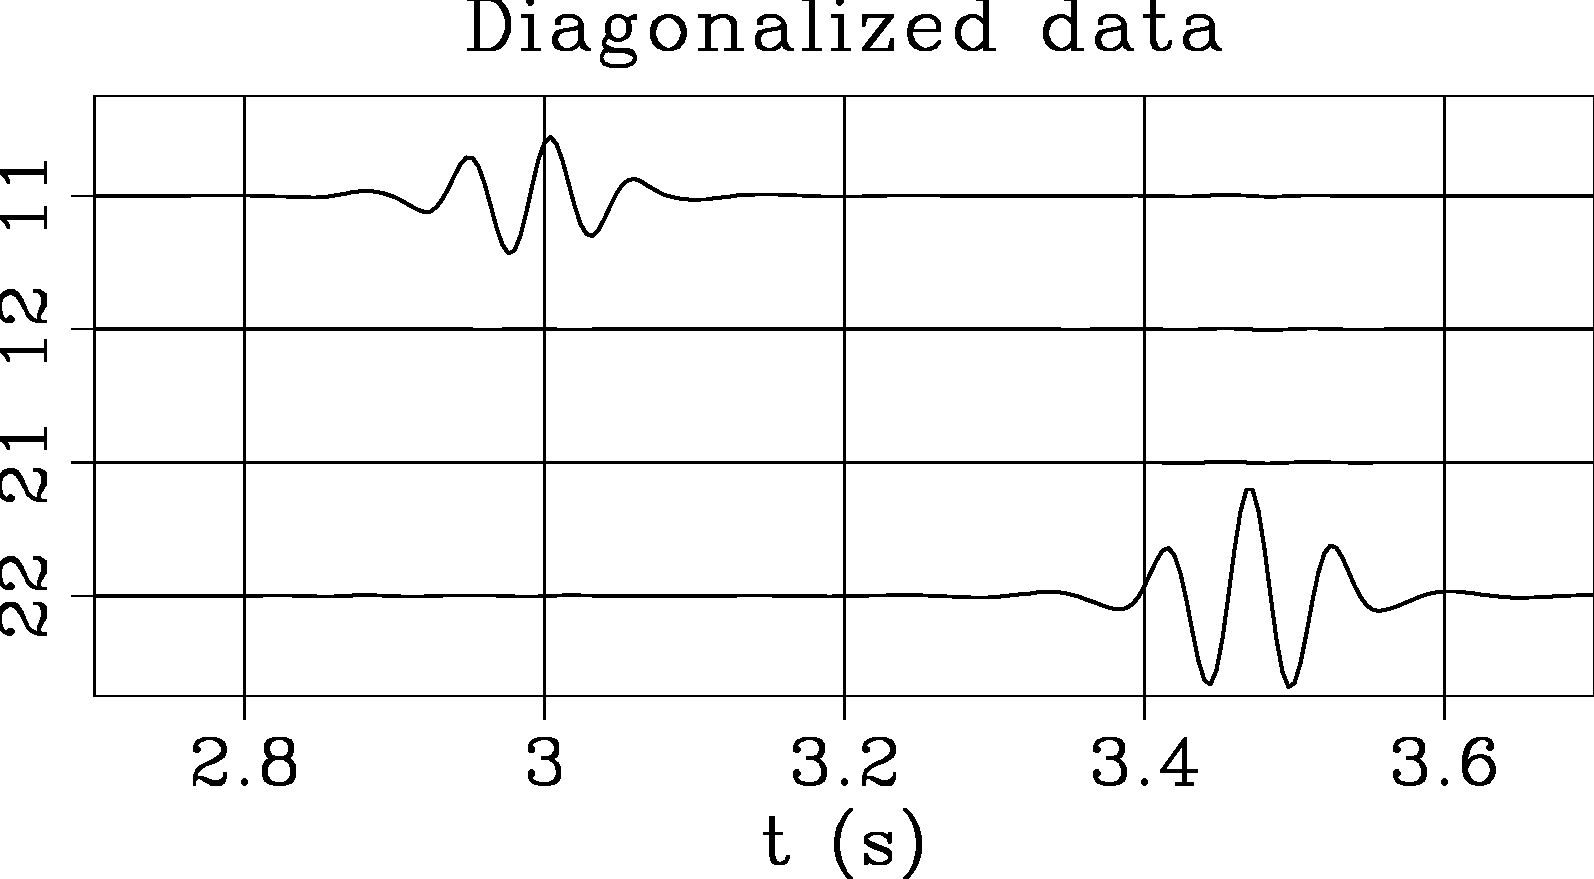
\includegraphics[width=\textwidth]{Fig/waves}
  \caption{First caption.}
  \label{fig:waves}
\end{figure}

Sometimes it is convenient to put two or more figures from different
files in an array (see Figure~\ref{fig:exph,exgr}). Individual plots
are Figures~\ref{fig:exph} and~\ref{fig:exgr}.

\begin{figure}
  \centering
  \subfigure[]{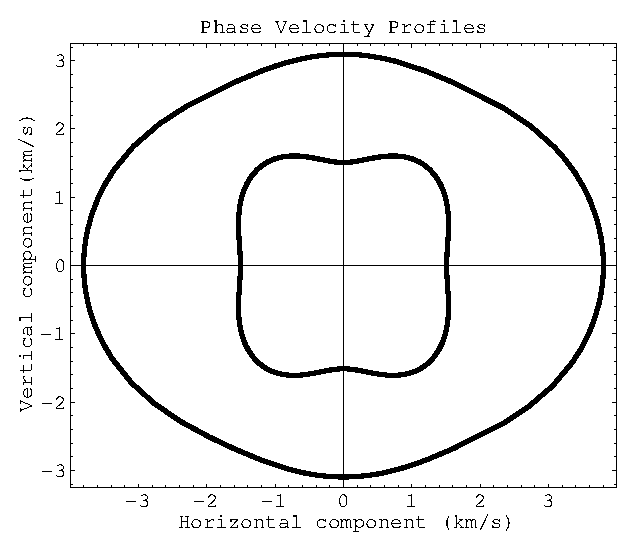
\includegraphics[width=0.4\textwidth]{Fig/exph}\label{fig:exph}}
  \subfigure[]{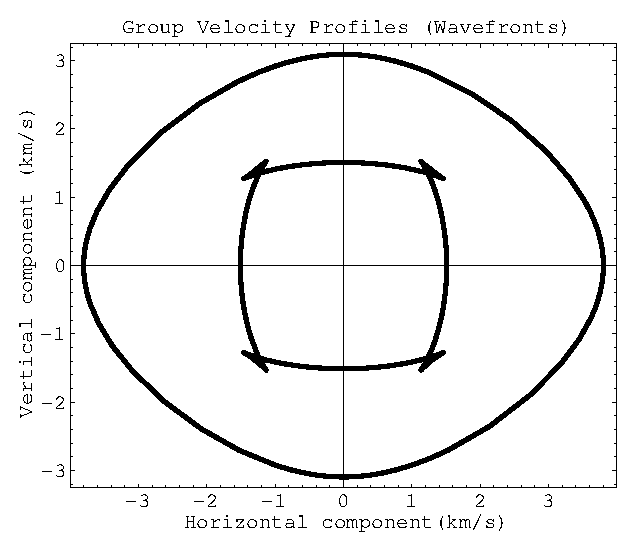
\includegraphics[width=0.4\textwidth]{Fig/exgr}\label{fig:exgr}}
  \caption{Second caption}
  \label{fig:exph,exgr}
\end{figure}

The first argument of the \texttt{multiplot} command specifies the
number of plots per row.

\subsection{Tables}

The discussion is summarized in Table~\ref{tbl:example}.

\begin{table}
  \centering
  \begin{tabular}{|c|c|c|}
    \hline
    \multicolumn{3}{|c|}{Table Example} \\
    \hline
    migration\rule[-2ex]{0ex}{5ex} & 
    $\omega \rightarrow k_z$ & $k_y^2+k-z^2\cos^2 \psi=4\omega^2/v^2$ \\
    \hline
    \parbox{1in}{zero-offset\\diffraction}\rule[-4ex]{0ex}{8ex} &
    $k_z\rightarrow\omega_0$ &
    $k_y^2+k_z^2=4\omega_0^2/v^2$ \\
    \hline
    DMO+NMO\rule[-2ex]{0in}{5ex} & $\omega\rightarrow\omega_0$ & $\frac{1}{4}
    v^2k_y^2\sin^2\psi+\omega_0^2\cos^2\psi=\omega^2$ \\
    \hline
    radial DMO\rule[-2ex]{0in}{5ex} & $\omega\rightarrow\omega_s$ &
    $\frac{1}{4}v^2k_y^2\sin^2\psi+\omega_s^2=\omega^2$\\
    \hline
    radial NMO\rule[-2ex]{0in}{5ex} & $\omega_s\rightarrow\omega_0$ &
    $\omega_0\cos\psi=\omega_s$\\
    \hline
  \end{tabular}
  \caption{Table caption}
  \label{tbl:example}
\end{table}

\begin{acknowledgments}
I wish to thank Ivan P\v{s}en\v{c}\'{\i}k and Fr\'ed\'eric Billette for having
names with non-English letters in them.  I wish to thank \cite{Cerveny} for
providing an example of how to make a bib file that includes an author
whose name begins with a non-English character and \cite{forgues96} for
providing both an example of referencing a Ph.D. thesis and yet more
non-English characters.
\end{acknowledgments}

\append{Appendix example}

According to the new SEG standard, appendices come before references.

\begin{equation}
\frac{\partial U}{\partial z} = 
\left\{
  \sqrt{\frac{1}{v^2} - \left[\frac{\partial t}{\partial g}\right]^2} +
  \sqrt{\frac{1}{v^2} - \left[\frac{\partial t}{\partial s}\right]^2}
\right\}
\frac{\partial U}{\partial t}
\label{eqn:partial}
\end{equation}
It is important to get equation~\ref{eqn:partial} right. See also
Appendix~\ref{equations}.

\append[equations]{Another appendix}

\begin{equation}
\frac{\partial U}{\partial z} = 
\left\{
  \sqrt{\frac{1}{v^2} - \left[\frac{\partial t}{\partial g}\right]^2} +
  \sqrt{\frac{1}{v^2} - \left[\frac{\partial t}{\partial s}\right]^2}
\right\}
\frac{\partial U}{\partial t}
\label{eqn:partial2}
\end{equation}
Too lazy to type a different equation but note the numeration.

The error comparison is provided in Figure~\ref{fig:errgrp}.

\begin{figure}
  \centering
  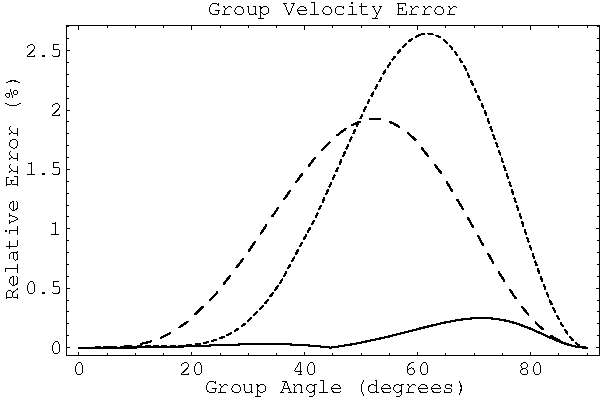
\includegraphics[width=0.8\textwidth]{Fig/errgrp}
  \caption{Third caption}
  \label{fig:errgrp}
\end{figure}

\append{The source of this document}

\verbatiminput{geophysics_example.ltx}

\append{The source of the bibliography}

\verbatiminput{example.bib}

\newpage

\bibliographystyle{seg}  % style file is seg.bst
\bibliography{example}

\end{document}
